The results consist of two parts:
\begin{itemize}
\item A benchmark of the impact of different parameters on the
  tracking performance, performed on artificial videos and evaluated
  programmatically
\item A test run on real data with the best performing parameters from
  the benchmark, evaluated manually
\end{itemize}

\section{Parameter Benchmark}

A benchmark was performed in order to identify how tracking
performance is affected by the different parameters. The benchmark was
performed on generated videos of artificial whiskers, which enabled
programmatic evaluation of the results since the correct shapes of the
whiskers, the \emph{ground truth}, were known.

The benchmarks were run on about 16 computers\footnote{This varied in
  time as other students also wanted access to the computers.} in the
computer halls Grå and Karmosin at KTH for two nights. The computers
were all equipped with 2.83 GHz quad-core Intel\textregistered \;
Core\texttrademark \; 2 Quad processors and 3.8 GiB of RAM, and were
running Ubuntu Linux 10.04.

\subsection{Test data}
\label{sec:test-data}

The test data consisted of a single generated video of artificial
whiskers. The video contained 6 whiskers and was 64 frames long. Each
whisker had length 200 and a random base shape $\Spline{\omega}$, with
$a_3, a_2, a_1$. Each $a_i$ was in the range $\left[0,
  \sigma_i\right)$, where $\sigma_3 = 1.6 \cdot 10^{-5}, \sigma_2 =
4\cdot 10^{-3}, \sigma_1 = 1$. Each whisker was then assigned a random
phase $d \in \left[0, 2\pi\right)$, and the shape at time step $t$ was
$\left(\Spline{\omega}\right) \sin(\frac{2\pi t}{30} + d)$.

The shape and the frequency $\frac{1}{30}$ were selected through
manual inspection of a video of real whiskers in order to make the
generated whiskers roughly realistic. The resulting whiskers were
roughly reminiscent of real whiskers, and 6 sample frames can be seen
in figure \ref{fig:benchmark-video}.

The database was generated with the same settings as the video, and
contained $2^{14} = 16384$ transitions. Each transition consisted of a
``from'' part $\tf$ and a ``to'' part $\tt$. $\tf$ was created by
generating a base state and phase in the same way as for the video,
and setting $t=0$. $\tt$ was created by taking $\tf$ and increasing
the phase by $\frac{2\pi}{30}$.

\begin{figure}
  \centering
  \begin{tabular}{ccc}
    \includegraphics[width=0.3\textwidth]{benchmark-video/frame-00000.png} &
    \includegraphics[width=0.3\textwidth]{benchmark-video/frame-00005.png} &
    \includegraphics[width=0.3\textwidth]{benchmark-video/frame-00010.png}\\
    Frame 0 & Frame 5 & Frame 10\\
    \includegraphics[width=0.3\textwidth]{benchmark-video/frame-00015.png} &
    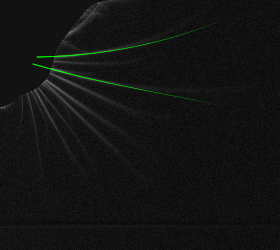
\includegraphics[width=0.3\textwidth]{benchmark-video/frame-00020.png} &
    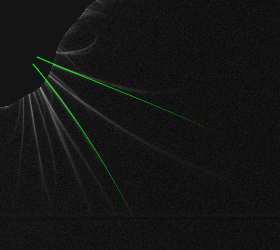
\includegraphics[width=0.3\textwidth]{benchmark-video/frame-00025.png}\\
    Frame 15 & Frame 20 & Frame 25
  \end{tabular}
  \caption{Sample frames from the testing video.}
  \label{fig:benchmark-video}
\end{figure}  


\subsection{Evaluated parameters}
The following parameters were evaluated:

\begin{description}
\item[n] Number of particles
\item[p] In which $\Lp$ space to compute $\Lpnorm{\tf - x_{t-1}}$ in
  the prediction step
\item[a] The exponent for the weights in the prediction step, $w =
  \Lpnorm{\tf - x_{t-1}}^{-a}$
\item[$\sigma$] Standard deviation modifier for the offset in the
  prediction step. Standard deviations for the $\omega^3, \omega^2$
  and $\omega$ terms are $\sigma\sigma_3, \sigma\sigma_2$ and
  $\sigma\sigma_1$, respectively.\footnote{See section
    \ref{sec:test-data} for the $\sigma_i$ values.}
\item[g] The exponent for the importance in the filtering step
\end{description}

Table \ref{tbl:testcases} shows the tested values. The values to test
were chosen for the following reasons:

\begin{description}
\item[n] 512 particles was the most the computer systems could handle
  in reasonable time. This was then scaled down to 64 as lower
  particle counts are, subjectively, quite uninteresting.
\item[p] The $\Lp$ norm computation implementation used only handled
  even values of $p$. Computation time increased rapidly with $p$, so
  $p=8$ was the highest value for which the computations could be done
  in time.
\item[a] The range was chosen to start from 1 because lower values
  would counteract the intended purpose of the parameter. The end 8
  was chosen since higher values were believed to restrict the
  prediction too much.
\item[$\sigma$] The max value 0.2 was selected so that each parameter
  could vary roughly a fifth of the parameter space in each
  direction. The other three were selected as lower, exponentially
  spaced points.
\item[g] The range was selected in the same way as that of $a$.
\end{description}

All value series were spaced exponentially since orders of magnitude
are most interesting in this benchmark.

\begin{table}
  \centering
  \begin{tabular}{c|l}
    Parameter & Values\\
    \hline
    $n$ & 64, 128, 256, 512\\
    $p$ & 2, 4, 8\\
    $a$ & 1, 2, 4, 8\\
    $\sigma$ & 0.025, 0.05, 0.1, 0.2\\
    $g$ & 1, 2, 4, 8
  \end{tabular}
  \caption{Specification of test cases.}
  \label{tbl:testcases}
\end{table}

\subsection{Benchmark procedure}

The benchmark was run on the test video for each combination of
parameters in table \ref{tbl:testcases}. The output from the benchmark
is an error matrix $\epsilon_{i,t}$, where index $i, t$ contains
$\Lpnorm[2]{Z_t - x_t}$, the $\Lp[2]$ distance between the ground
truth and estimated shape for whisker $i$ at time $t$. From this, a
list $\epsilon_i$ was computed as the root mean square of
$\epsilon_{i,t}$ in the $t$ direction. Finally, the maximum value in
$\epsilon_i$ was selected as the \emph{error} $\epsilon$ of that
run. This gives us the error tensor

\begin{equation}
  E_{n,p,a,\sigma,g} = \argmax{i} \sqrt{\frac{\sum\limits_t
      \epsilon_{i,t}^2}{64} } ~ \forall \left(n, p,
    a, \sigma, g\right).
\end{equation}

However, some tests took a very long time to run, and therefore some
did not finish in time. This included all tests for $n=512$ and $p=8$,
some of whose running times were observed to exceed 12 hours. These
test cases and the ones specified in table \ref{tbl:unfinished-runs}
were not included in the analysis.

\begin{table}[h]
  \centering
  \begin{tabular}{ccccc}
    $n$ & $p$ & $a$ & $\sigma$ & $g$\\
    \hline
    64 & 8 & 4 & 0.05 & 8\\
    64 & 8 & 8 & 0.05 & 1\\
    64 & 8 & 8 & 0.1 & 2\\
    64 & 8 & 8 & 0.025 & 4\\
    512 & 2 & 4 & 0.025 & 4\\
    512 & 2 & 4 & 0.05 & 4\\
    512 & 2 & 4 & 0.1 & 4\\
    512 & 4 & 1 & 0.2 & 8
  \end{tabular}
  \caption{Unfinished test runs. Omitted are $\left(512, 8, a, \sigma,
      g\right) ~ \forall a, \sigma, g$.}
  \label{tbl:unfinished-runs}
\end{table}

Note that the absolute magnitude of the error $\epsilon$ is irrelevant
- it is the ratios between these errors that is interesting. One could
argue for instead using the relative error $\Lpnorm[2]{Z_t - x_t} /
\Lpnorm[2]{Z_t}$, but the relative error is misleading here. The
reason is that a deviation from a very bent whisker would then be
considered better than the same deviation from a very straight
whisker. Therefore the absolute error is used for the analysis.

Since the error tensor is five-dimensional, displaying all of its
contents is not feasible. Instead the index $\left(n_0, p_0, a_0,
  \sigma_0, g_0\right)$ for which $E_{n_0, p_0, a_0, \sigma_0,g_0}$ is
minimized was used as the common point of the following plots. Using
this index, the the cross sections
\begin{IEEEeqnarray}{rCl}
  E_{p,a} &=& E_{n_0, p, a, \sigma_0, g_0} ~ \forall p, a\\
  E_{\sigma,g} &=& E_{n_0, p_0, a_0, \sigma, g} ~ \forall \sigma, g\\
  E_n &=& E_{n, p_0, a_0, \sigma_0, g_0} ~ \forall n
\end{IEEEeqnarray}
were extracted and plotted.

Also investigated was the effect of computing $E$ using the $\Lp[4]$
and $\Lp[8]$ norms, in order to see if this had some correlation to
the choice of $p$. However, the resulting $E_{p,a}$ and $E_{\sigma,g}$ for
$\Lp[2], \Lp[4]$ and $\Lp[8]$ all had the same qualitative behaviour,
so the $\Lp[4]$ and $\Lp[8]$ versions of $E$ are omitted from this
report.

\subsection{Results}

The minimum of $E_{n,p,a,\sigma,g}$ was found to be 38.18 for
\begin{equation*}
  n=512, p=2, a=2, g=4, s=0.2.
\end{equation*}

Figures \ref{fig:Epa-maxerr-L2} and \ref{fig:Esg-maxerr-L2} show
$E_{p,a}$ and $E_{\sigma,g}$, respectively. Figures
\ref{fig:Epa-maxerr-L2-nobig} and \ref{fig:Esg-maxerr-L2-nobig} show
the same graphs, but with the dominant points removed. Figure
\ref{fig:En-maxerr-L2} shows $E_n$.

\begin{figure}[p]
  \centering
  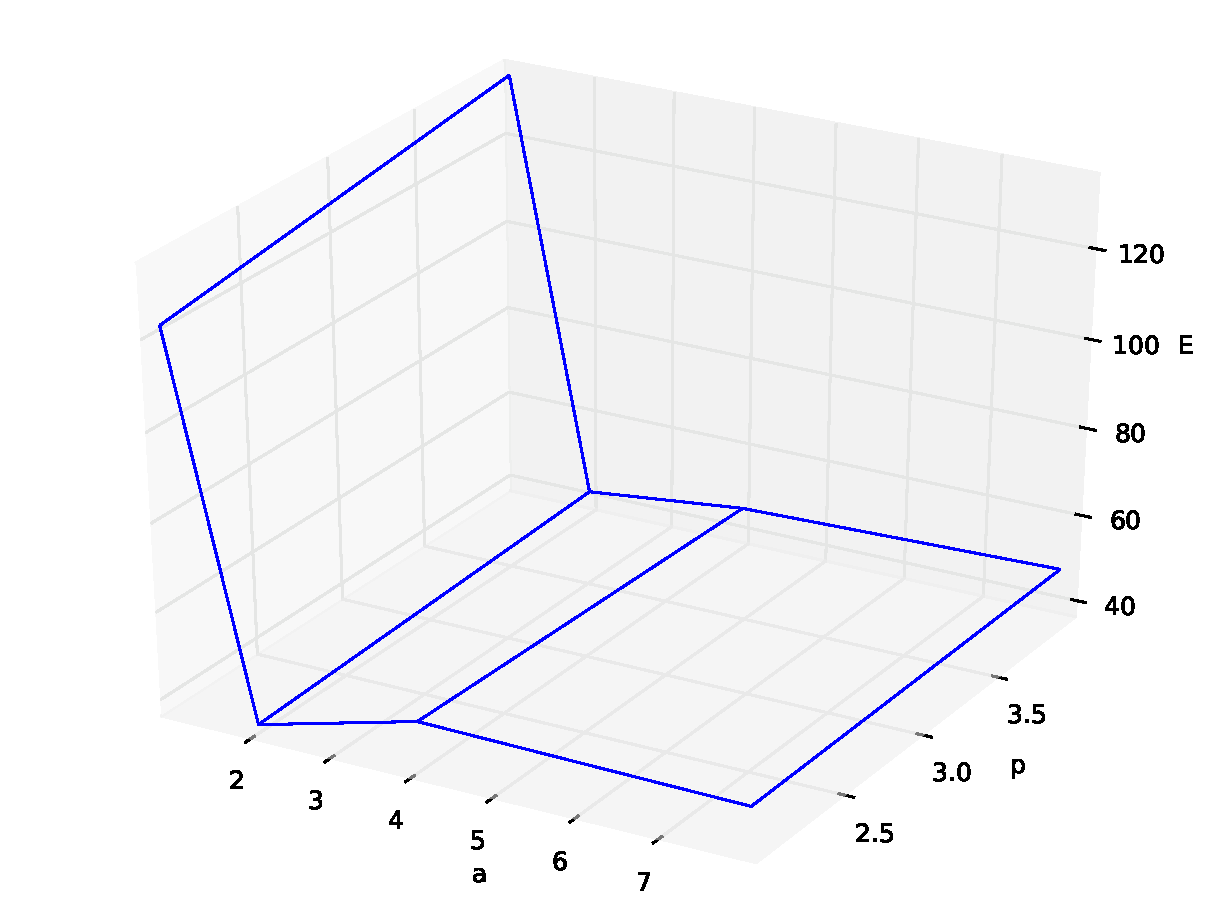
\includegraphics[width=0.8\textwidth]{benchmark/Epa-maxerr-L2.pdf}
  \caption{$E_{p,a}$.}
  \label{fig:Epa-maxerr-L2}
\end{figure}

\begin{figure}[p]
  \centering
  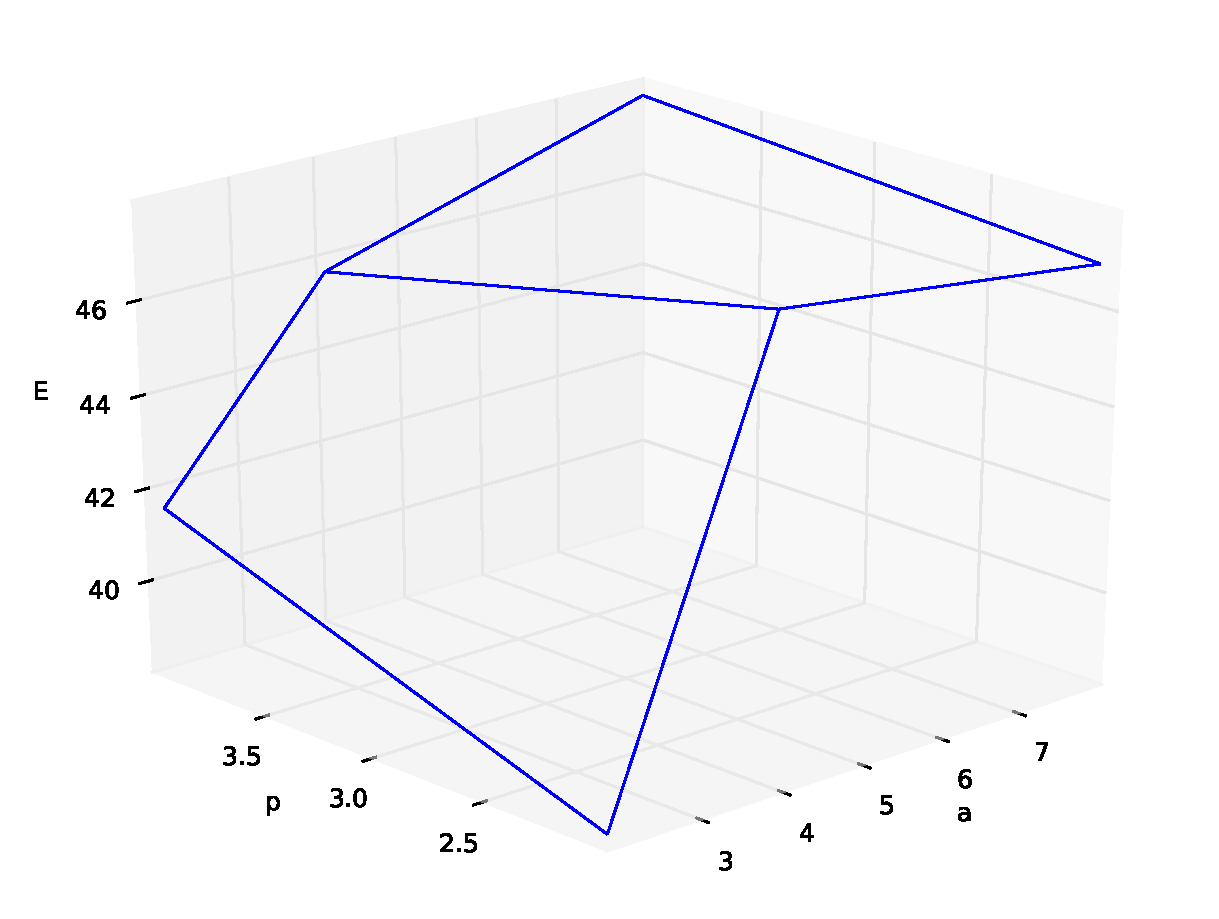
\includegraphics[width=0.8\textwidth]{benchmark/Epa-maxerr-L2-nobig.pdf}
  \caption{$E_{p,a}$ with dominant points removed. Notice that the
    plot has been rotated so that the $p$ axis now extends to the
    left.}
  \label{fig:Epa-maxerr-L2-nobig}
\end{figure}

\begin{figure}[p]
  \centering
  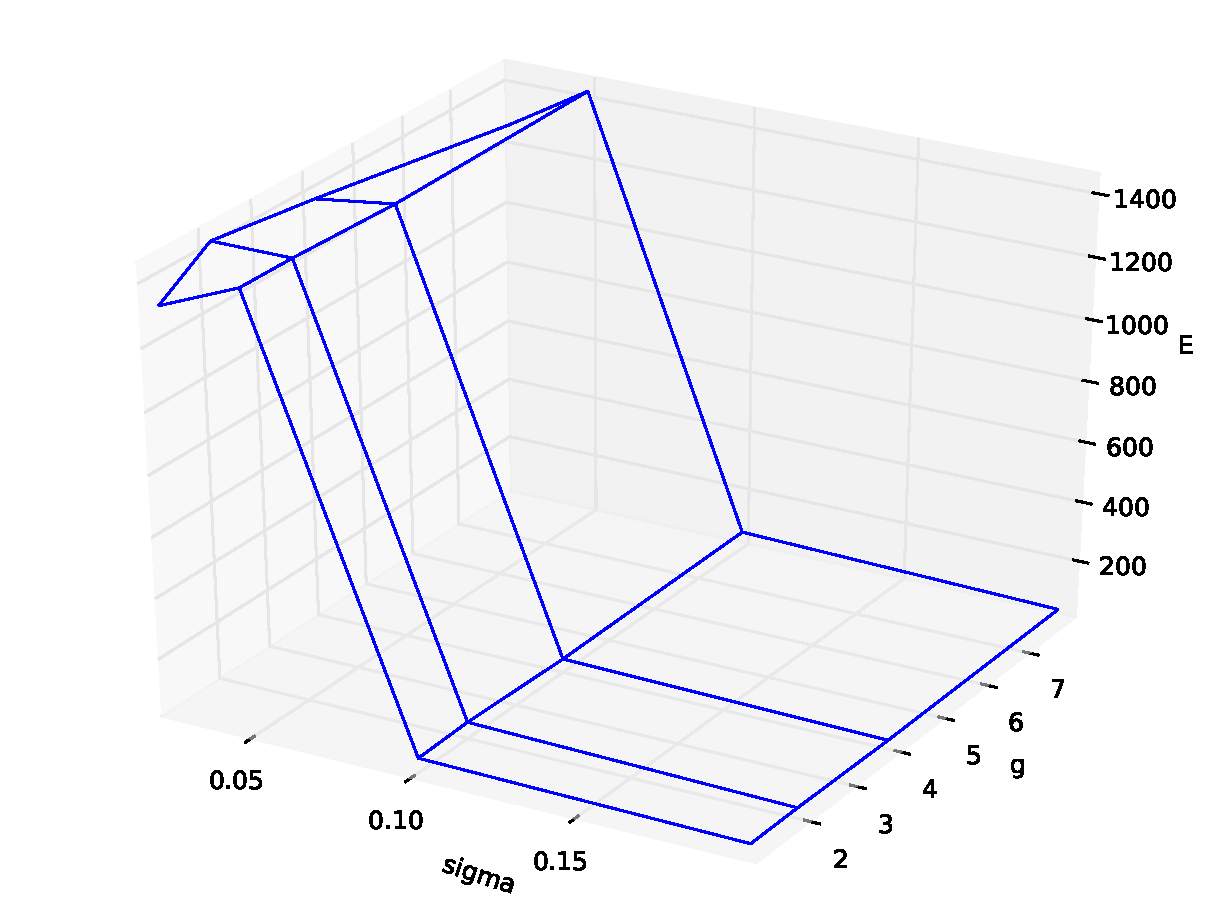
\includegraphics[width=0.8\textwidth]{benchmark/Esg-maxerr-L2.pdf}
  \caption{$E_{\sigma,g}$.}
  \label{fig:Esg-maxerr-L2}
\end{figure}

\begin{figure}[p]
  \centering
  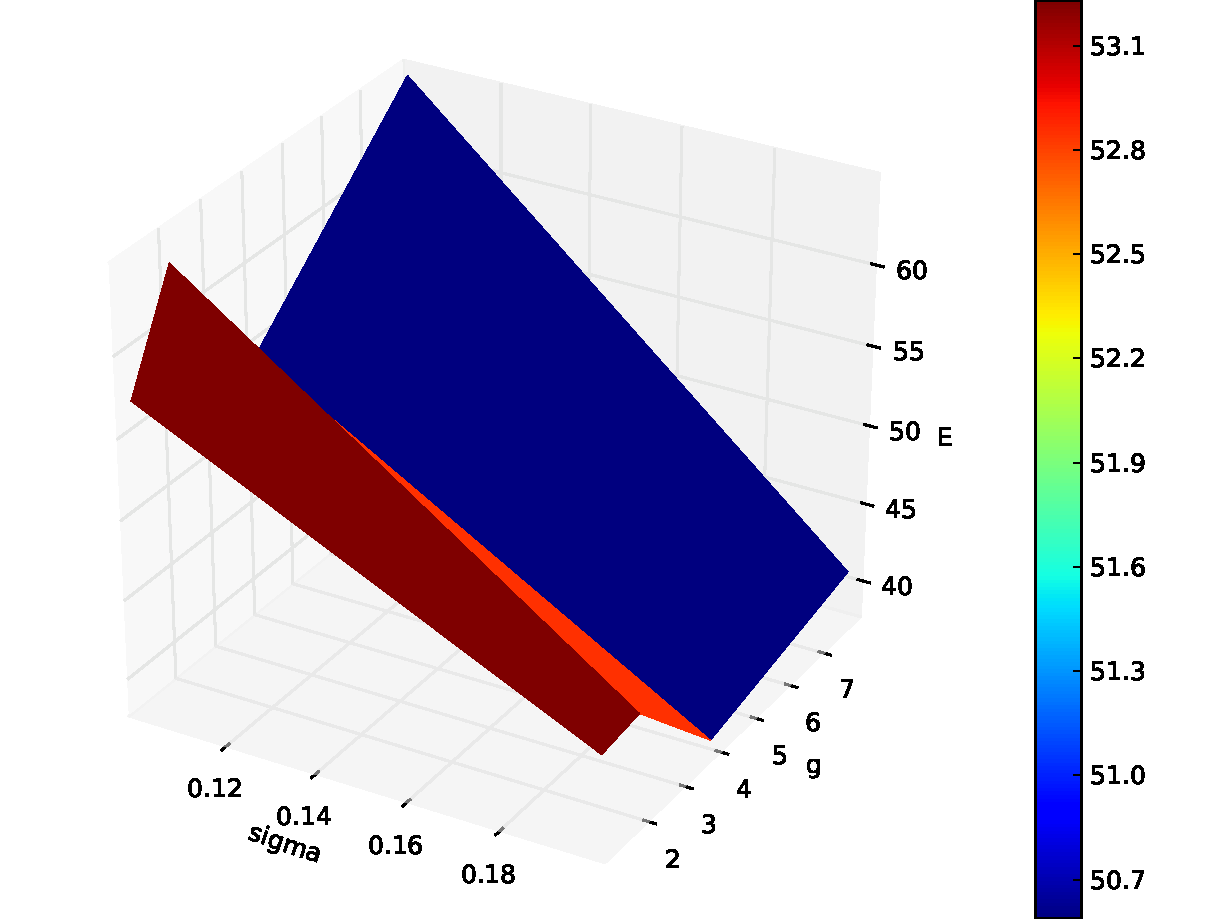
\includegraphics[width=0.8\textwidth]{benchmark/Esg-maxerr-L2-nobig.pdf}
  \caption{$E_{\sigma,g}$ with dominant points removed.}
  \label{fig:Esg-maxerr-L2-nobig}
\end{figure}

\begin{figure}[p]
  \centering
  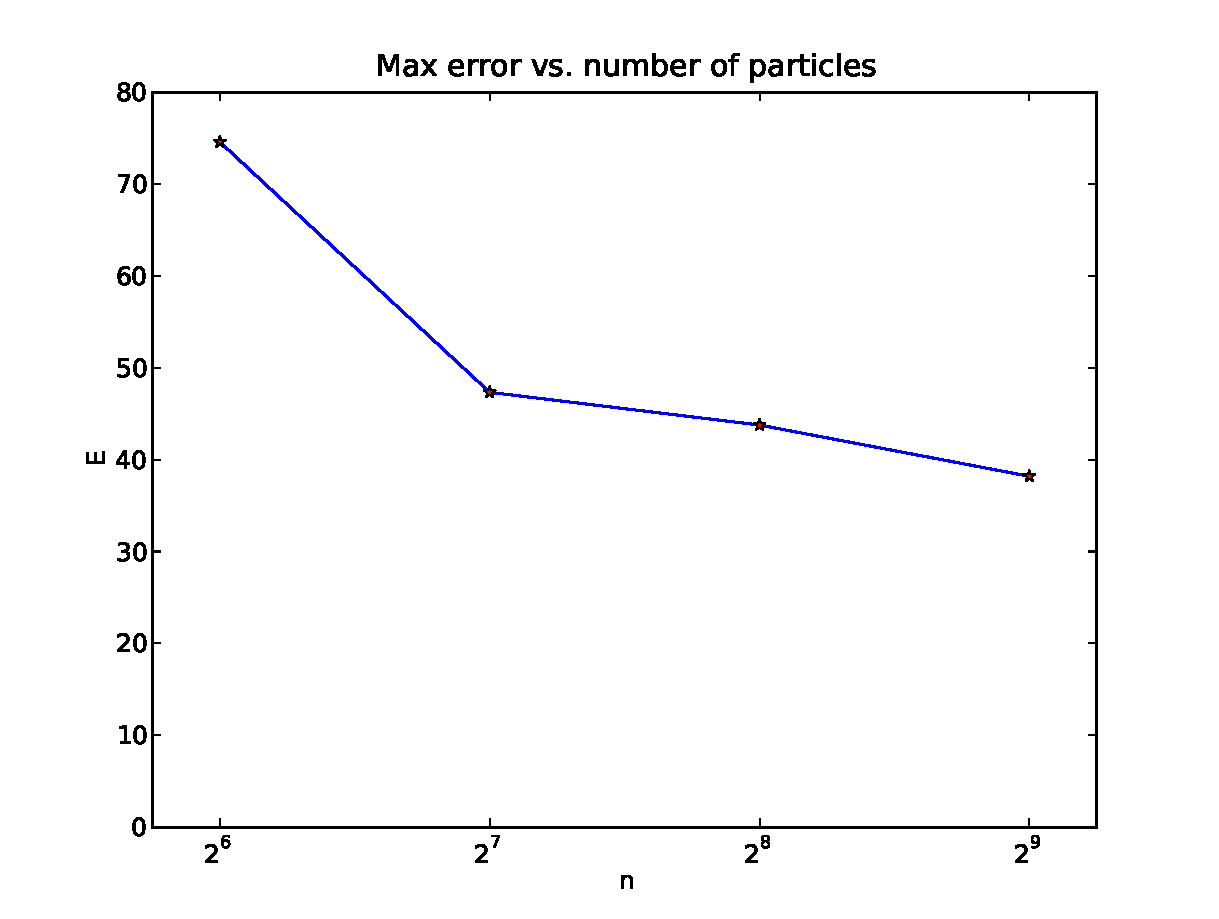
\includegraphics[width=0.8\textwidth]{benchmark/En-maxerr-L2.pdf}
  \caption{$E_n$. Note the logarithmic scale of $n$.}
  \label{fig:En-maxerr-L2}
\end{figure}


\section{Run on real data}

The parameters $\left(n_0, p_0, a_0, \sigma_0, g_0\right)$ from the
parameter benchmark were used for running the tracker on a real
whisker video of 131 frames. The performance was evaluated manually.

Figure \ref{fig:rtracking} shows the first 18 frames, including the
manually initialized start frame. Green lines are the estimated shapes
of the whiskers.. The following figures show a selection of images
from the tracking sequence. Figure \ref{fig:rtracking-jump} shows how
the model of the lower whisker ``jumps'' to another whisker further
down the array. Figure \ref{fig:rtracking-jump-coincide} shows another
jump, this time resulting in both models coinciding. Figure
\ref{fig:rtracking-double-jump} shows how both models
simultaneously jump to other whiskers, the top being a smaller whisker.

\begin{figure}[p]
  \centering
  \begin{tabular}{ccc}
    \includegraphics[width=0.3\textwidth]{tracking/frame-00000.png} &
    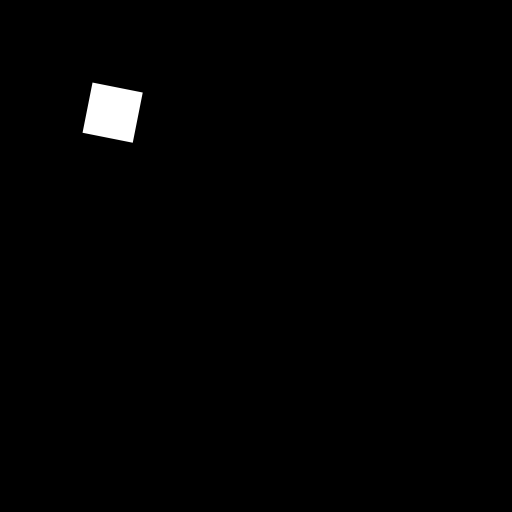
\includegraphics[width=0.3\textwidth]{tracking/frame-00001.png} &
    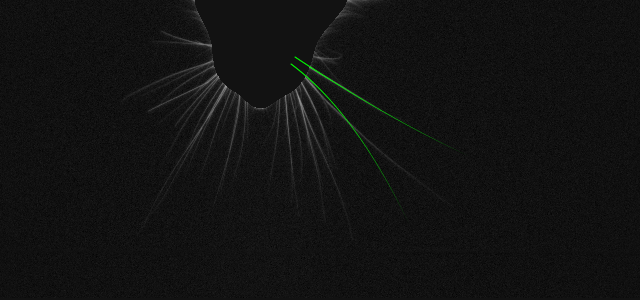
\includegraphics[width=0.3\textwidth]{tracking/frame-00002.png}\\
    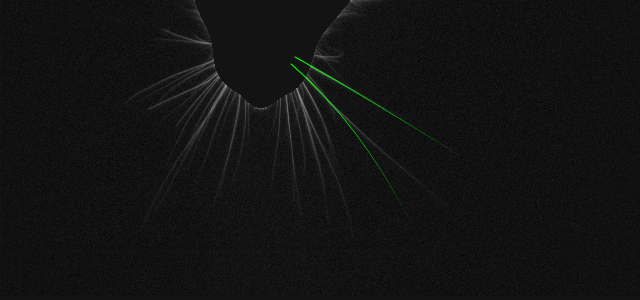
\includegraphics[width=0.3\textwidth]{tracking/frame-00003.png} &
    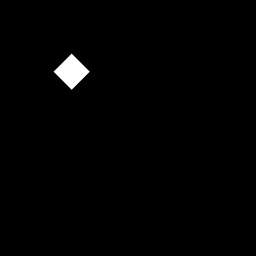
\includegraphics[width=0.3\textwidth]{tracking/frame-00004.png} &
    \includegraphics[width=0.3\textwidth]{tracking/frame-00005.png}\\
    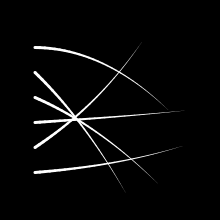
\includegraphics[width=0.3\textwidth]{tracking/frame-00006.png} &
    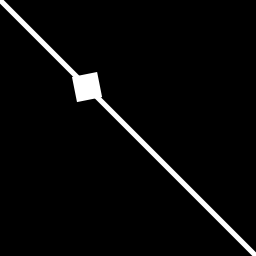
\includegraphics[width=0.3\textwidth]{tracking/frame-00007.png} &
    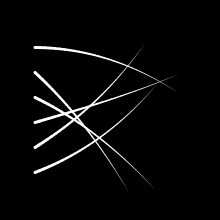
\includegraphics[width=0.3\textwidth]{tracking/frame-00008.png}\\
    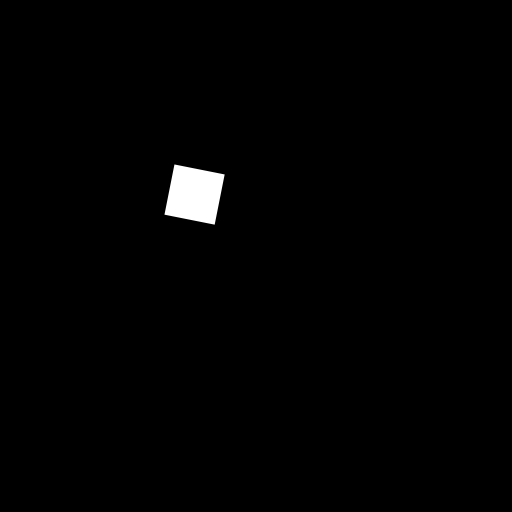
\includegraphics[width=0.3\textwidth]{tracking/frame-00009.png} &
    \includegraphics[width=0.3\textwidth]{tracking/frame-00010.png} &
    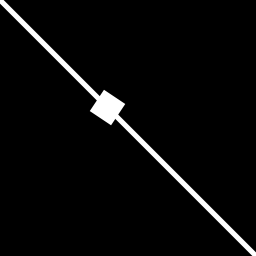
\includegraphics[width=0.3\textwidth]{tracking/frame-00011.png}\\
    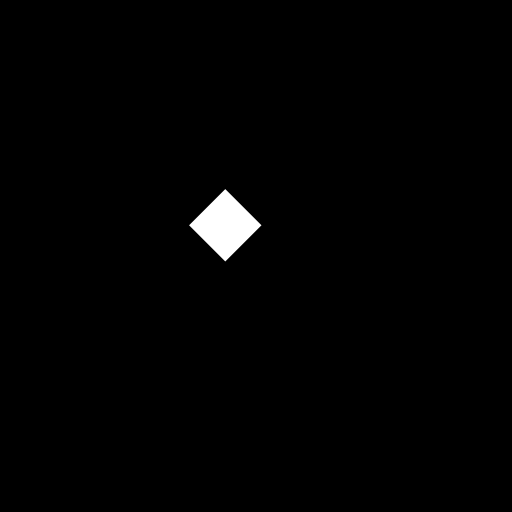
\includegraphics[width=0.3\textwidth]{tracking/frame-00012.png} &
    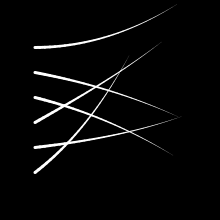
\includegraphics[width=0.3\textwidth]{tracking/frame-00013.png} &
    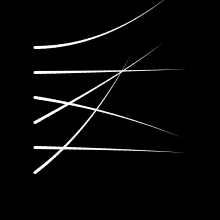
\includegraphics[width=0.3\textwidth]{tracking/frame-00014.png}\\
    \includegraphics[width=0.3\textwidth]{tracking/frame-00015.png} &
    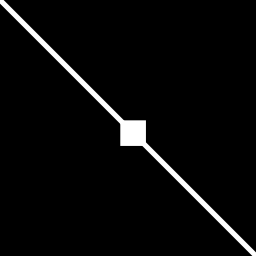
\includegraphics[width=0.3\textwidth]{tracking/frame-00016.png} &
    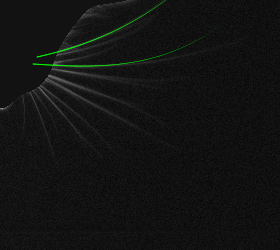
\includegraphics[width=0.3\textwidth]{tracking/frame-00017.png}\\
  \end{tabular}
  \caption{The 18 first frames from tracking results on real data.}
  \label{fig:rtracking}
\end{figure}

\begin{figure}[p]
  \centering
  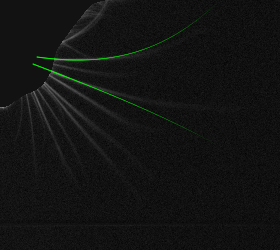
\includegraphics[width=0.45\textwidth]{tracking/frame-00021.png}
  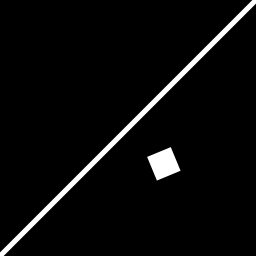
\includegraphics[width=0.45\textwidth]{tracking/frame-00022.png}
  \caption{Frames 22 and 23. The model of the lower whisker ``jumps''
    to another whisker.}
  \label{fig:rtracking-jump}
\end{figure}

\begin{figure}[p]
  \centering
  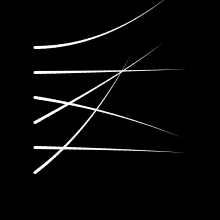
\includegraphics[width=0.45\textwidth]{tracking/frame-00044.png}
  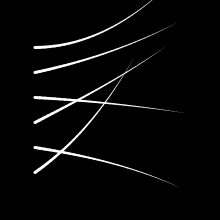
\includegraphics[width=0.45\textwidth]{tracking/frame-00045.png}
  \caption{Frames 45 and 46. The model of the lower whisker jumps to
    another whisker, this time coinciding with the top model.}
  \label{fig:rtracking-jump-coincide}
\end{figure}

\begin{figure}[p]
  \centering
  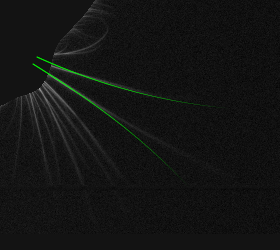
\includegraphics[width=0.45\textwidth]{tracking/frame-00121.png}
  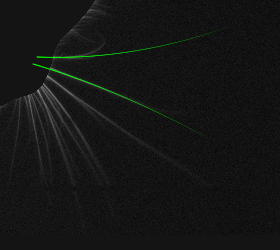
\includegraphics[width=0.45\textwidth]{tracking/frame-00122.png}
  \caption{Frames 122 and 123. Both models jump simultaneously.}
  \label{fig:rtracking-double-jump}
\end{figure}


\begin{comment}
\begin{verbatim}
Mål:
  - Någon form av slutsats huruvida det är rimligt att fortsätta
undersöka detta
    - Identifiera problem och svårigheter
      - Vad är svårare? Försök kvantifiera svårigheter hos problemen
    - Utvärdera prestanda hos algoritmen
      - Tid
      - Resultat

Rapporten:
  - Går det att skala problemet? Undersök.
  - Jämför lösningar
\end{verbatim}

The measures that will be used as fitness of the parameters:
    \begin{description}
        \item[$\int{||\epsilon(t)||_{L^p}}dt$]
            integrating over time the the difference
            with the ground truth (do this for L{1:10} and see if it correlates with
            the p choosed (to see how much it deviates from the ground truth)
        \item[$\int{\Response{x_t}{I_t}{\phi} }dt$] 
            integrating over time the response
            for the choosed hypothesis (to see how the different image transformation
            affects the results, that is if it only follows what it thinks is best
            (phi))
        \item[Subjective] 4 image samples
    \end{description}
And all this are done for all 4 benchmark videos.

<<more shall come>>

%"There are many metrics by which a model may be assessed." - Encyclopedia

%Tillvägagångsätt:
%1. Since we have prior knowledge about the effect off varying the parameters n,N
%they will firstly be set to a sufficently large value.
%2. A partion of the test-matrix will then be evaluated by ... parameter group 
\end{comment}